\documentclass[13pt]{beamer}

\usefonttheme{professionalfonts}
\usetheme{Antibes}
\setbeamertemplate{footline}[frame number]

\usepackage[
    backend=biber,
    style=alphabetic,
    sorting=ynt
]{biblatex}
\addbibresource{../bib/bibliografia.bib}

\makeatletter
\setbeamertemplate{footline}
{
    \leavevmode%
    \hbox{%
        \begin{beamercolorbox}[wd=.333333\paperwidth,ht=2.25ex,dp=1ex,center]{author in head/foot}%
            \usebeamerfont{author in head/foot}\insertshortauthor
        \end{beamercolorbox}%
        \begin{beamercolorbox}[wd=.333333\paperwidth,ht=2.25ex,dp=1ex,center]{title in head/foot}%
            \usebeamerfont{title in head/foot}\insertshorttitle
        \end{beamercolorbox}%
        \begin{beamercolorbox}[wd=.333333\paperwidth,ht=2.25ex,dp=1ex,right]{date in head/foot}%
            \usebeamerfont{date in head/foot}\insertshortdate{}\hspace*{2em}
            \insertframenumber{} / \inserttotalframenumber\hspace*{2ex} 
        \end{beamercolorbox}}%
        \vskip0pt%
    }
    \makeatother

%% Itemize bullet head

% set the itemize item symbol as a triangle
\setbeamertemplate{itemize item}{\scriptsize$\blacktriangleright$}
% set the itemize subitem symbol as a diamond
\setbeamertemplate{itemize subitem}{\scriptsize$\diamond$}
% set the itemize subsubitem symbol as a circle with a dot
\setbeamertemplate{itemize subsubitem}{\scriptsize$\odot$}

\usepackage[portuguese]{babel}
\usepackage{csquotes}
\usepackage{graphicx}
\usepackage{amsmath, mathtools, mathrsfs, amssymb}
\usepackage{verbatim}
\usepackage{pgfplots}
\usepackage{xcolor}
    \pgfplotsset{compat=1.18}
    \pgfplotsset{lua debug}
\usepackage{tikz}
\usepackage{graphicx}
\usetikzlibrary{positioning, matrix}
\usepackage{bm}
\usepackage{hyperref}
\hypersetup{
    colorlinks=true,
    citecolor=blue,
    linkcolor=blue,
    filecolor=magenta,
    urlcolor=blue,
    pdfpagemode=FullScreen,
}

%% Supress overful hbox warnings until this lenght
\hfuzz=3.22pt 
\vfuzz=4.6pt 

\DeclareMathOperator{\proj}{proj \ }
\renewcommand{\arraystretch}{1.4}
\newcommand{\transpose}{\mathsf{T}}

%% Environments

\theoremstyle{plain} % default
\newtheorem{teo}{Teorema}[section]
\newtheorem*{teo*}{Teorema}
\newtheorem{lem}{Lema}[section]
\newtheorem*{lem*}{Lema}
\newtheorem{prop}{Proposição}[section]
\newtheorem{cor}[teo]{Corolário}
\newtheorem*{cor*}{Corolário}
\newtheorem*{axiom}{Axioma}

\newtheorem*{TAU}{Teorema da Aproximação Universal}
\newtheorem*{Riesz}{Teorema da Representação de Riesz}

\theoremstyle{definition}
\newtheorem{defn}{Definição}[section]
\newtheorem*{defn*}{Definição}
\newtheorem{conj}{Conjectura}[section]
\newtheorem{exmp}{Exemplo}[section]
\newtheorem{rem}{Observação}[section]
\newtheorem*{rem*}{Observação}

\theoremstyle{remark}
% \newtheorem*{note}{Nota}
\newtheorem{case}{Caso}


% Macros

\renewcommand{\Re}{\text{Re}}

\newcommand{\bfx}{\bm{x}}
\newcommand{\bfX}{\bm{X}}
\newcommand{\bfy}{\bm{y}}
\newcommand{\bfz}{\bm{z}}
\newcommand{\bfw}{\bm{w}}
\newcommand{\bfv}{\bm{v}}

\newcommand{\bvx}{\vec{\bm{x}}}


\newcommand{\bH}{\mathbb{H}}
\newcommand{\K}{\mathbb{K}}
\newcommand{\I}{\mathbb{I}}

\DeclarePairedDelimiter{\dotprod}{\langle}{\rangle}

\DeclareMathOperator{\rk}{rk}
\DeclareMathOperator{\intt}{int}
\DeclareMathOperator{\diam}{diam}
\DeclareMathOperator{\rref}{rref}
\DeclareMathOperator{\vspan}{span}
\DeclareMathOperator{\lin}{Lin}
\DeclareMathOperator{\supp}{supp}



\DeclareMathOperator{\posto}{posto}

% Swap the definition of \abs* and \norm*, so that \abs
% and \norm resizes the size of the brackets, and the 
% starred version does not.

\usepackage{global-macros}

\title[Deep Galerkin Method]{Deep Galerkin Method \\ {\normalsize Resolvendo EDPs Numericamente com Redes Neurais}}
\author[C. Lins]{Caio Lins}
\institute[EMAp]{FGV - EMAp}
\date[EMAp 2021]{Novembro 2021}
\titlegraphic{
\includegraphics[height=0.8cm]{../figuras/fgv_logo.png}}

\begin{comment}
    TODO:
        -- Ler papers citados pelo DGM
\end{comment}

\begin{document}

\maketitle

\begin{frame}{Sumário}
    \tableofcontents
\end{frame}

\AtBeginSection[]{
    \begin{frame}{Sumário}
        \tableofcontents[currentsection]
    \end{frame}
}

\section{Equações Diferenciais Parciais}

\begin{frame}{Formulação do problema}
    \begin{block}{EDP com condições iniciais e de fronteira}
        Dados
        \begin{itemize}
            \item \( \Omega \subseteq \R^{ d } \) e \( T > 0 \) -- domínio
            \item \( u_{ 0 } : \Omega \to \R \) -- condição inicial
            \item \( g : [0, T] \times \partial \Omega \to \R \) -- condição de fronteira,
        \end{itemize}
        \visible<2->{queremos encontrar \( u : [0, T] \times \Omega \to \R \) tal que
        \begin{equation*}
            \begin{cases}
                \partial_{ t } u ( t, \bfx ) + \mathcal{L} u ( t, \bfx ) = 0, &( t, \bfx ) \in [0, T] \times \Omega \\
                u ( 0, \bfx ) = u_{ 0 } ( \bfx ), &\bfx \in \Omega \\
                u ( t, \bfx ) = g ( t, \bfx ), &( t, \bfx ) \in [0, T] \times \partial \Omega
            \end{cases}
    \end{equation*}}
    \end{block}

\end{frame}

\begin{frame}{Formulação do problema}
    Aqui \( \mathcal{L} \) é um operador diferencial como, por exemplo, o laplaciano \( \nabla^2 \):
    \begin{equation*}
        \nabla^2 u = \frac{ \partial^2 u }{ \partial x_{ 1 }^2 } + \cdots + \frac{ \partial^2 u }{ \partial x_{ d }^2 }
    .\end{equation*}
\end{frame}

%% TODO: Colocar imagens para ilustrar métodos non-network
\begin{frame}{Métodos numéricos}
    \begin{itemize}
        \item<1-> A solução numérica de EDPs é um desafio substancial.
        \item<2-> Métodos numéricos non-network:
        \begin{itemize}
            \item<3-> \href{https://en.wikipedia.org/wiki/Finite_difference_method}{\emph{Métodos de diferenças finitas}}

                Aproxima os valores da solução \( u ( t, \bfx ) \) em um \emph{grid} utilizando uma equação de recorrência.

                \visible<4->{Por exemplo, para a equação do calor \( \partial_{ t } u = \partial_{ xx } u \):
                    \begin{equation*}
                        u ( t + \Delta t, \bfx ) \approx u ( t, \bfx ) + \mu [
                            u ( t, \bfx + \Delta \bfx ) - 2 u ( t, \bfx ) + u ( t, \bfx - \Delta \bfx )
                        ]
                    .\end{equation*}}
                \item<5-> \href{https://en.wikipedia.org/wiki/Finite_element_method}{\emph{Métodos de elementos finitos}}

                Utiliza um espaço de funções de dimensão finita para aproximar a solução.
                Por exemplo, funções lineares ou polinomiais por partes.

                Também faz uso de um \emph{grid}.
        \end{itemize}
    \end{itemize}
\end{frame}

\begin{frame}{Métodos Numéricos}
    \begin{figure}
        \begin{center}
            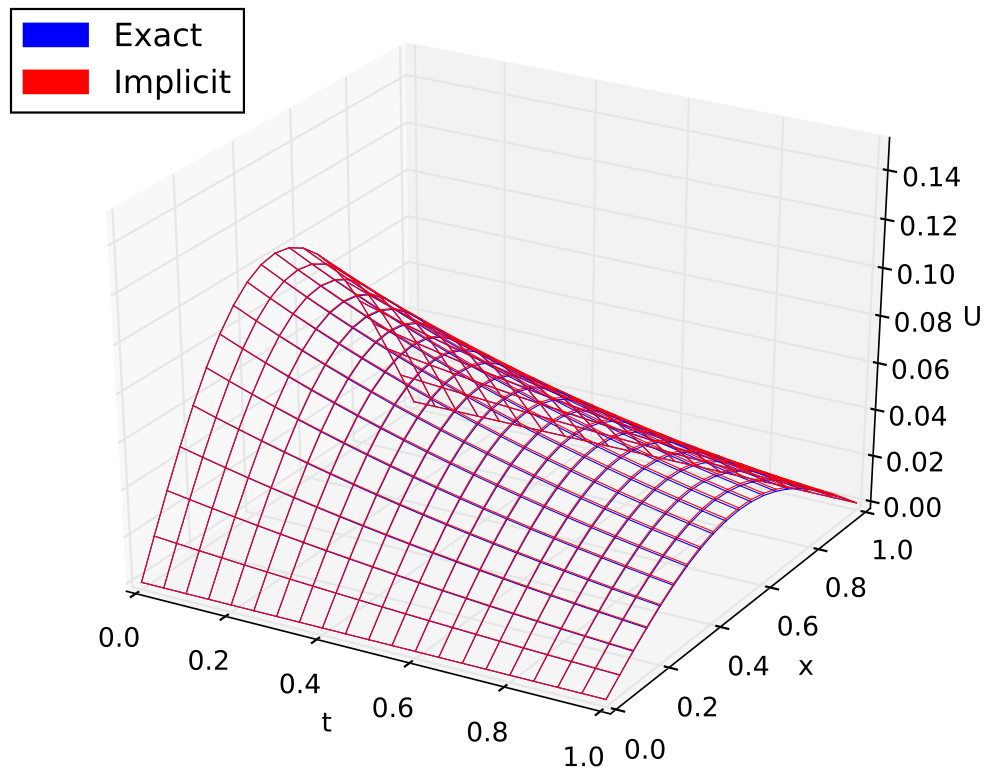
\includegraphics[width=.6\textwidth]{../figuras/fd-grid.png}
        \end{center}
        Exemplo de \emph{grid} aplicado no método de diferenças finitas.
    \end{figure}
\end{frame}


\begin{frame}{Métodos Numéricos}
    \begin{itemize}
        \item<1-> Principal problema: a necessidade do \emph{grid}.
        \item<2-> Número de pontos no \emph{grid} cresce exponencialmente com o número de dimensões espaciais.
        \item<3-> Métodos envolvendo Deep Learning passaram a contornar esse problema.
    \end{itemize}
\end{frame}

\section{Redes Neurais e EDPs}

\begin{frame}{Ideia Principal}
    \begin{itemize}
        \item<1-> Vamos tentar aproximar a solução da EDP em \( [0, T] \times \Omega \) com uma rede neural \( f ( t, \bfx, \theta ) \)
            \begin{itemize}
                \item<2-> Essa ideia faz sentido, pois redes neurais são aproximadores universais de funções contínuas \cite{hornik91}.
            \end{itemize}
        \item<3-> Função de perda teórica, com três partes:
            \begin{align*}
                J ( f ) = &\int_{ [0, T] \times \Omega } \norm{ \partial_{ t } f ( t, \bfx, \theta ) + \mathcal{L} f ( t, \bfx, \theta ) }^2 \ \mathrm{d}\nu_{ 1 } \\
                &+ \int_{ [0, T] \times \partial \Omega } \norm{ f ( t, \bfx, \theta ) - g ( t, \bfx ) }^2 \ \mathrm{d}\nu_{ 2 } \\
                &+ \int_{ \Omega } \norm{ f ( 0, \bfx, \theta ) - u_{ 0 } ( \bfx ) }^2 \ \mathrm{d}\nu_{ 3 }
            ,\end{align*}
            onde \( \nu_{ 1 }, \nu_{ 2 }, \nu_{ 3 } \) são medidas finitas.
    \end{itemize}
\end{frame}

\begin{frame}{Ideia Principal}
    \begin{itemize}
        \item<1-> Na prática, para calcular a perda em um conjunto de pontos
            \begin{equation*}
                \begin{cases}
                    ( t_{ i }, \bfx_{ i } ) \subset [0, T] \times \Omega, \\
                    ( \tau_{ i }, \bfy_{ i } ) \subset [0, T] \times \partial \Omega, \\
                    \bfw_{ i } \subset \Omega,
                \end{cases}
            \end{equation*}
            \( i = 1, \dots, n \), utilizamos o MSE:
            \begin{align*}
                G ( f ) = &\frac{ 1 }{ n } \sum_{ i=1 }^{ n } \abs{ \partial_{ t } f ( t_{ i }, \bfx_{ i }, \theta ) + \mathcal{L} f ( t_{ i }, \bfx_{ i }, \theta ) }^2 \\
                    &+ \frac{ 1 }{ n } \sum_{ i=1 }^{ n } \abs{ f ( \tau_{ i }, \bfy_{ i }, \theta ) - g ( \tau_{ i }, \bfy_{ i } ) }^2 \\
                    &+ \frac{ 1 }{ n } \sum_{ i=1 }^{ n } \abs{ f ( 0, \bfw_{ i }, \theta ) - u_{ 0 } ( \bfw_{ i } ) }^2
            .\end{align*}
    \end{itemize}
\end{frame}

\begin{frame}{Primeiros Trabalhos}
    \begin{figure}[htb]
        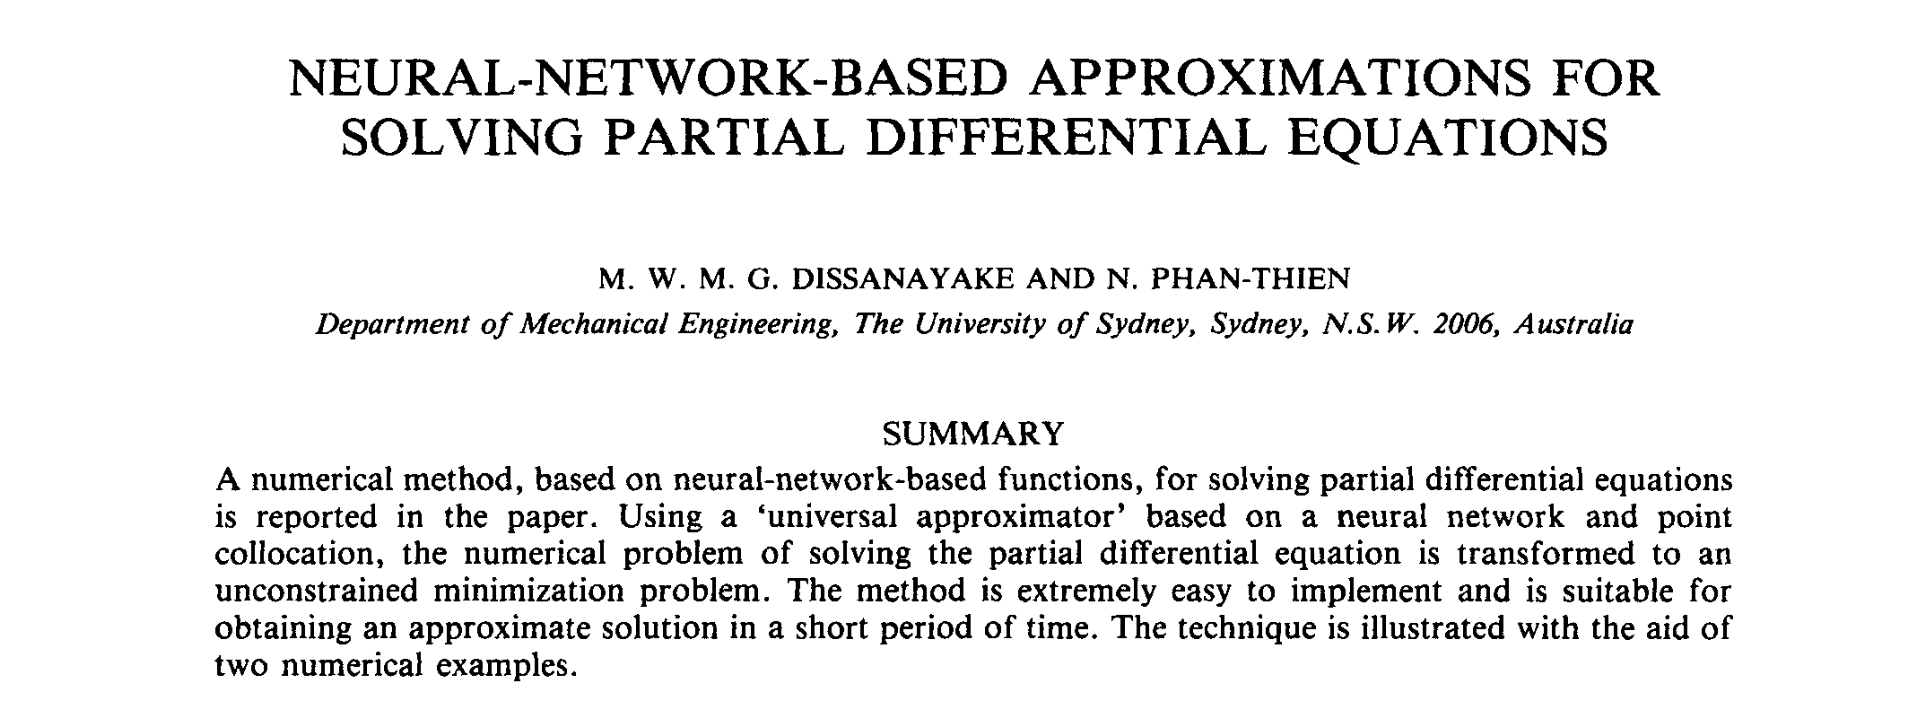
\includegraphics[width=\textwidth]{../figuras/seminal-1994.png}
    \end{figure}
    \cite{dissanayake94} utiliza essa ideia para solucionar equações bidimensionais definidas em \( \Omega = [0, 1]^2 \).
\end{frame}


\begin{frame}{Primeiros Trabalhos}
    Características principais:
    \begin{itemize}
        \item<1-> Uso de NNs do tipo feedforward como aproximadores.
        \item<2-> Otimização feita utilizando um método quasi-Newton.
        \item<3-> Gradientes aproximados utilizando diferenças finitas.
        \item<4-> Pontos de treino são tomados de um \emph{grid} no domínio.
    \end{itemize}
\end{frame}

\begin{frame}{Primeiros Trabalhos}
    \begin{figure}[htb]
        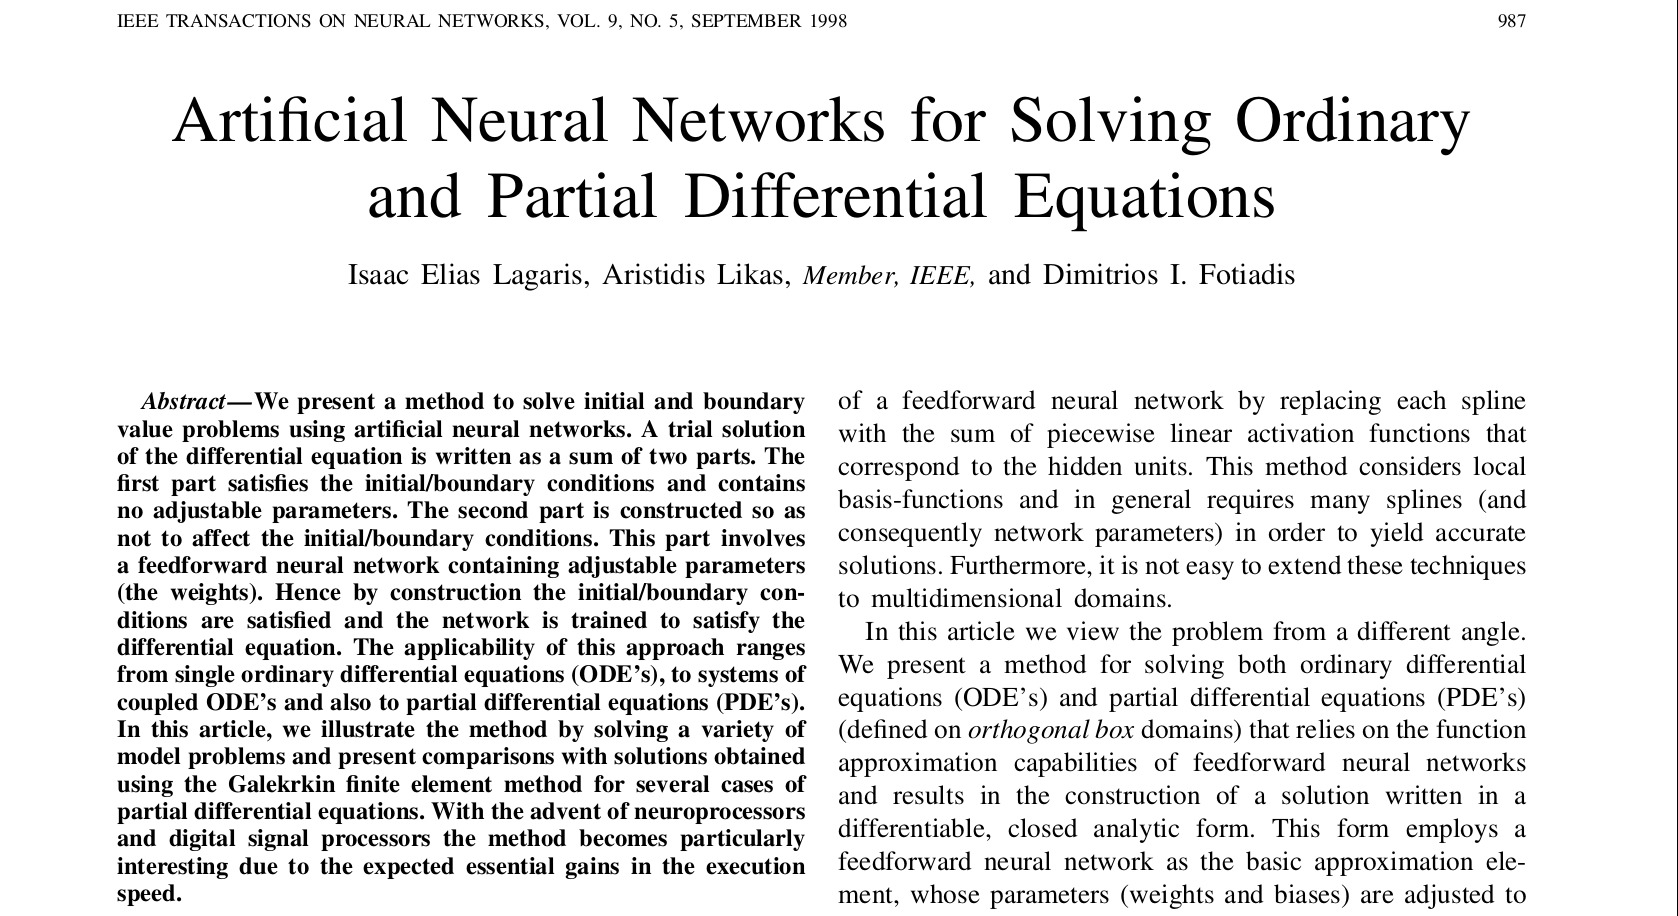
\includegraphics[width=.8\textwidth]{../figuras/seminal-1998.png}
    \end{figure}
    \cite{lagaris98} emprega esse método para solucionar EDOs, bem como EDPs definidas em cubos unitários.
\end{frame}

\begin{frame}{Primeiros Trabalhos}
    Principais diferenças:
    \begin{itemize}
        \item<1-> Solução não é exclusivamente uma rede neural.
            Se \( \Psi_{ \theta } \) é a solução aproximada parametrizada por \( \theta \), temos
            \begin{equation*}
                \Psi_{ \theta } ( \bvx ) = A ( \bvx ) + F ( \bvx, f ( \bvx, \theta ) )
            ,\end{equation*}
            onde \( f ( \bvx, \theta ) \) é a rede neural.

            \visible<2->{A ideia é que \( A ( \bvx ) \) não tenha parâmetros e satisfaça condições de fronteira.
                O termo \( F ( \bvx, f ( \bvx, \theta ) ) \) é encarregado fazer \( \Psi_{ \theta } \) obeder a EDP/EDO.
            }
    \end{itemize}
\end{frame}

\begin{frame}{Primeiros Trabalhos}
    Principais diferenças:
    \begin{itemize}
        \item<1-> Por exemplo, considerando a EDO:
            \begin{equation*}
                u' ( x ) = g ( x, u )
            ,\end{equation*}
            com condição inicial \( \Psi ( 0 ) = A \), a solução é escrita como
            \begin{equation*}
                \Psi_{ \theta } ( x ) = A + x f ( x, \theta )
            .\end{equation*}
        \item<2-> Além disso, passa a utilizar diferenciação automática.
    \end{itemize}
\end{frame}

\begin{frame}{Primeiros Trabalhos}
    Entretanto:
    \begin{itemize}
        \item<1-> Rede utilizada ainda é uma MLP.
        \item<2-> Otimização continua quasi-Newton.
        \item<3-> \emph{Grid} de treinamento se mantém.
    \end{itemize}
\end{frame}

\begin{frame}{Desenvolvimentos Mais Recentes}
    \begin{figure}[htb]
        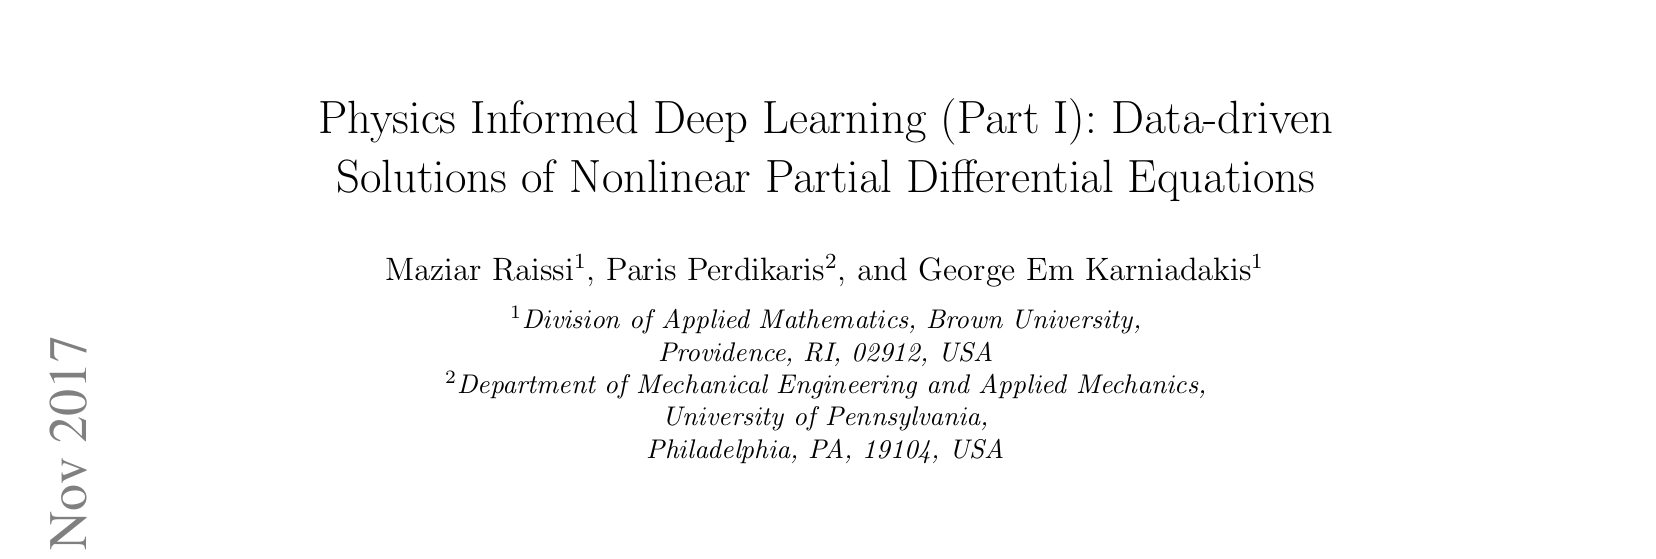
\includegraphics[width=\textwidth]{../figuras/pinn.png}
    \end{figure}
    \cite{raissi17} cunham o termo \emph{Physics Informed Neural Network -- PINN}
\end{frame}

\begin{frame}{Desenvolvimentos Mais Recentes}
    \begin{itemize}
        \item<1-> Uma PINN não necessariamente está relacionada a uma EDP.
        \item<2-> A ideia é incorporar informações vindas da física no processo de treinamento e, assim, fazer um uso mais eficiente dos dados disponíveis.
            \begin{itemize}
                \item Em sistemas físicos reais, o custo da aquisição de dados muitas vezes é demasiadamente elevado.
            \end{itemize}
        \item<3-> Entretanto, nos exemplos desse artigo especificamente, a ideia é incorporar a EDP na função de perda, como já descrevemos.
    \end{itemize}
\end{frame}

\begin{frame}{Desenvolvimentos Mais Recentes}
    Como agora o objetivo é ter a possibilidade de usar dados coletados, o conjunto de treino é um pouco diferente:
    \begin{itemize}
        \item<2-> Poucos pontos são tomados nas condições iniciais.
            \begin{itemize}
                \item \( 100 \) pontos, por exemplo.
            \end{itemize}
        \item<3-> A maior parte do conjunto de treino é tomada no interior de \( [0, T] \times \Omega \).
            \begin{itemize}
                \item E.g. \( 10 000 \) pontos distribuídos aleatoriamente.
            \end{itemize}
        \item<4-> Ou seja, não há mais um \emph{grid}.
            Os pontos no interior do domínio são amostrados uma única vez antes de começar o treinamento.
    \end{itemize}
\end{frame}

\begin{frame}{Desenvolvimentos Mais Recentes}
    \begin{itemize}
        \item<1-> Rede utilizada ainda é uma MLP, porém agora com mais camadas.
        \item<2-> Fizeram uso da diferenciação automática do Tensorflow.
        \item<3-> O algoritmo de otimização ainda é quasi-Newton.
    \end{itemize}
\end{frame}

\section{Deep Galerkin Method -- DGM}

\begin{frame}{Principais Características}
    \begin{figure}[htb]
        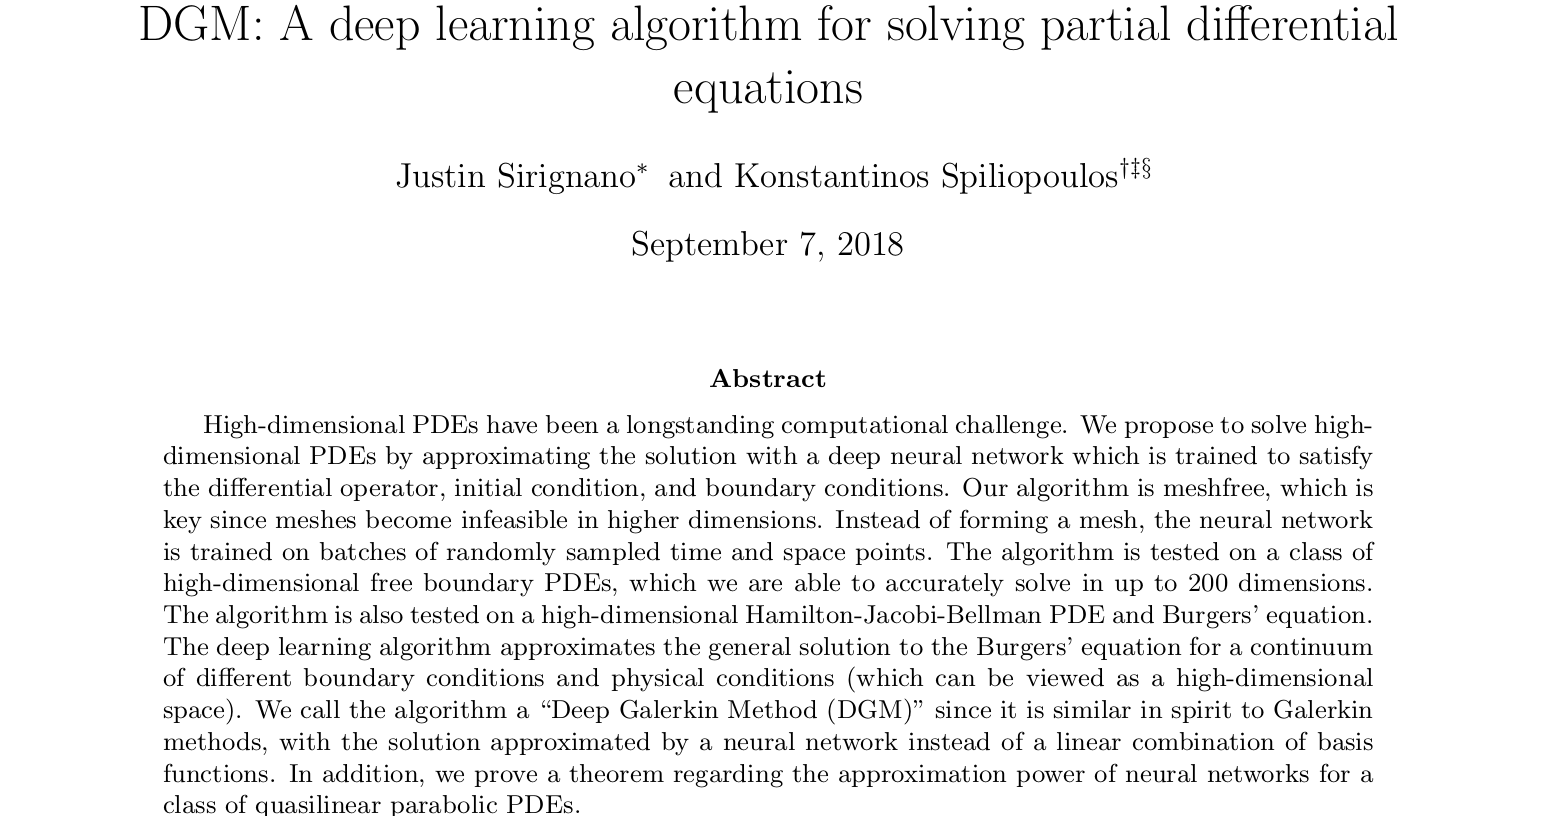
\includegraphics[width=.75\textwidth]{../figuras/dgm.png}
    \end{figure}
    \cite{sirignano18} Criaram um algoritmo que reúne as ideias até então apresentadas e faz algumas adições.
    Também provaram resultados teóricos sobre solucionar EDPs com redes neurais.
\end{frame}

\begin{frame}{Principais Características}
    \begin{itemize}
        \item<1-> \emph{Arquitetura da rede}:

            A arquitetura utiliza um mecanismo de \emph{gating} inspirado em redes do tipo LSTM/Highway \cite{hochreiter97} \cite{srivastava15}.

        \item<2-> \emph{Conjunto de treino}:

            Para realizar \textbf{cada update nos parâmetros} são amostrados novos pontos no domínio da EDP (1000, por exemplo).

            O treino passa a ser contado em termos de \emph{sampling stages} e não de épocas.
    \end{itemize}
\end{frame}

\begin{frame}{O Algoritmo}
    No \( n \)-ésimo \emph{sampling stage}:
    \begin{itemize}
        \item<1-> Gerar um conjunto de pontos \( s_{ n } \) pertencentes às três regiões de interesse: \( [0, T] \times \Omega, [0, T] \times \partial \Omega \) e \( \Omega \).
        \item<2-> Calcular o MSE: \( G ( \theta_{ n }, s_{ n } ) \)
        \item<3-> Atualizar os parâmetros com o gradiente da perda:
            \begin{equation*}
                \theta_{ n+1 } = \theta_{ n } - \alpha_{ n } \nabla_{ \theta } G ( \theta_{ n }, s_{ n } )
            \end{equation*}
            (na realidade, utilizamos o algoritmo ADAM).
    \end{itemize}
\end{frame}

\begin{frame}{Outras Adições}
    \begin{itemize}
        \item<1-> Treino \textbf{altamente paralelizado}:

            Realizado em 6 GPUs usando \emph{asynchronous stochastic gradient descent} \cite{dean12}.
            \begin{figure}[htb]
                    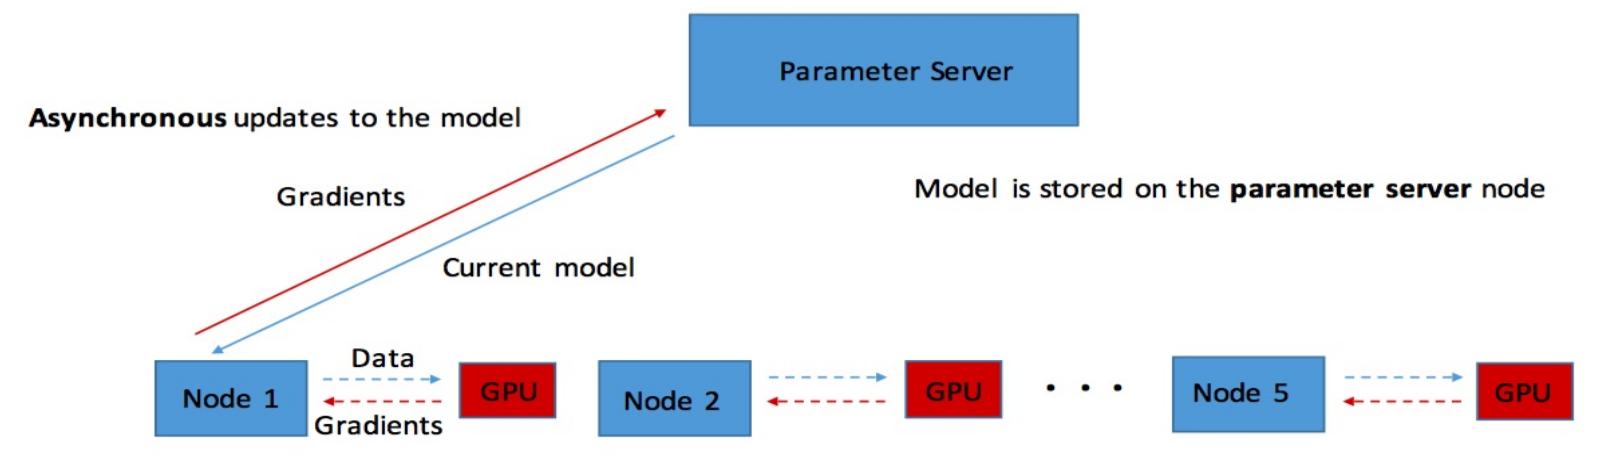
\includegraphics[width=.8\textwidth]{../figuras/asynchronous-sgd.png}
            \end{figure}

        \item<2-> Algoritmo Monte-Carlo para cálculo de segundas derivadas.

            Se torna mais rápido que diferenciação automática em muitas dimensões.
    \end{itemize}
\end{frame}

\begin{frame}{Arquitetura}
    \begin{itemize}
        \item Camada inicial densa, seguida por \( L \) camadas do tipo Highway/LSTM-like, terminando com uma transformação afim (aqui, \( \bvx = ( t, \bfx ) \)):
            \begin{align*}
                S^{ 1 } &= \sigma ( W^{ 1 } \bvx + b^{ 1 } ) \\
                Z^{ \ell } &= \sigma \left(
                    U^{ z, \ell } \bvx + W^{ z, \ell } S^{ \ell } + b^{ z, \ell }
                \right), \ell = 1, \dots, L, \\
                G^{ \ell } &= \sigma \left(
                    U^{ g, \ell } \bvx + W^{ g, \ell } S^{ \ell } + b^{ g, \ell }
                \right), \ell = 1, \dots, L, \\
                R^{ \ell } &= \sigma \left(
                    U^{ r, \ell } \bvx + W^{ r, \ell } S^{ \ell } + b^{ r, \ell }
                    \right), \ell = 1, \dots, L, \\
                H^{ \ell } &= \sigma \left(
                    U^{ h, \ell } \bvx + W^{ h, \ell } \left(
                        S^{ \ell } \odot R^{ \ell }
                    \right) + b^{ h, \ell }
                \right), \ell = 1, \dots, L, \\
                S^{ \ell + 1 } &= \left(
                        \bm{1} - G^{ \ell }
                    \right) \odot H^{ \ell } + Z^{ \ell } \odot S^{ \ell } \\
                    f ( t, \bfx, \theta ) &= W S^{ L + 1 } + b
            \end{align*}
    \end{itemize}
\end{frame}

\begin{frame}{Arquitetura}
    \begin{itemize}
        \item<1-> Temos \( L + 1 \) camadas ocultas, cada uma com \( M \) nós.
        \item<2-> A função \( \sigma : \R^{ M } \to \R^{ M } \) é uma não-linearidade elemento a elemento:
            \begin{equation*}
                \sigma ( \bfz ) = \left(
                    \varphi ( z_{ 1 } ), \varphi ( z_{ 2 } ), \dots, \varphi ( z_{ M } )
                \right)
            ,\end{equation*}
            onde \( \varphi : \R \to \R \) é uma função de ativação não linear.
        \item<3-> Parâmetros:
        \begin{align*}
            \theta = \Big\{ &W^{ 1 }, b^{ 1 },
                \left(
                    U^{ z, \ell }, W^{ z, \ell }, b^{ z, \ell }
                \right)_{ \ell = 1 }^{ L },
                \left(
                    U^{ g, \ell }, W^{ g, \ell }, b^{ g, \ell }
                \right)_{ \ell = 1 }^{ L }, \\
                            &\left(
                                U^{ r, \ell }, W^{ r, \ell }, b^{ r, \ell }
                            \right)_{ \ell = 1 }^{ L },
                            \left(
                                U^{ h, \ell }, W^{ h, \ell }, b^{ h, \ell }
                        \right)_{ \ell = 1 }^{ L }, W, b \Big\}
        .\end{align*}
    \end{itemize}
\end{frame}

\begin{frame}{Arquitetura}
    Sugestões dos autores:
    \begin{itemize}
        \item \( L = 3 \).
        \item \( M = 50 \).
        \item \( \varphi = \tanh \).
    \end{itemize}
\end{frame}

\begin{frame}{Avanços e Problemas}
    \begin{itemize}
        \item<1-> Autores reportaram alta precisão na solução de equações com até 200 dimensões -- ausência de \emph{grid}.
        \item<2-> Provaram um Teorema demonstrando a possibilidade de aproximar as soluções de uma classe de EDPs parabólicas quasilineares usando redes neurais.

    \end{itemize}
\end{frame}

\begin{frame}{Avanços e Problemas}
    Lembremos da função de perda teórica para uma rede \( f ( t, \bfx, \theta ) \):
    \begin{align*}
        J ( f ) = &\int_{ [0, T] \times \Omega } \norm{ \partial_{ t } f ( t, \bfx, \theta ) + \mathcal{L} f ( t, \bfx, \theta ) }^2 \ \mathrm{d}\nu_{ 1 } \\
        &+ \int_{ [0, T] \times \partial \Omega } \norm{ f ( t, \bfx, \theta ) - g ( t, \bfx ) }^2 \ \mathrm{d}\nu_{ 2 } \\
        &+ \int_{ \Omega } \norm{ f ( 0, \bfx, \theta ) - u_{ 0 } ( \bfx ) }^2 \ \mathrm{d}\nu_{ 3 }
    .\end{align*}
\end{frame}

\begin{frame}{Avanços e Problemas}
    \begin{teo*}
        Seja \( \mathfrak{C}^{ n } \) a classe de redes neurais com uma camada oculta e \( n \) nós.
        Seja \( f^{ n } \in \mathfrak{C}^n \) tal que \( J ( f^{ n } ) \) é mínimo em \( \mathfrak{C}^{ n } \).
        Sob certas condições, existe \( f^{ n } \in \mathfrak{C}^{ n } \) tal que
        \begin{equation*}
            J ( f^{ n } ) \to 0 \text{ quando } n \to \infty
        \end{equation*}
        e
        \begin{equation*}
            f^{ n } \to u \text{ quando } n \to \infty
        .\end{equation*}
        em \( L^{ \rho } ( [0, T] \times \Omega ) \), com \( \rho < 2 \).
    \end{teo*}
\end{frame}

\begin{frame}{Avanços e Problemas}
    Principais questões pendentes:
    \begin{itemize}
        \item<1-> Dificuldade de implementação.
        \item<2-> Falta de garantias teóricas.
    \end{itemize}
\end{frame}


\begin{frame}[allowframebreaks]{Referências}
    \printbibliography
\end{frame}

\end{document}

